\ifx \globalmark \undefined %% This is default.
	\documentclass[twoside,openright,11pt,a4paper]{report}

%\compiler avec xelatex
%\usepackage[applemac]{inputenc}
\usepackage[T1]{fontenc}
\usepackage[utf8]{inputenc} %latin1 est possible
%\usepackage[latin1]{inputenc} %latin1 est possible
\usepackage[UKenglish]{babel}
\usepackage{lettrine}

%\usepackage[text={13cm,20cm},centering]{geometry}
\usepackage [squaren, Gray, mediumqspace]{SIunits}
\usepackage [top=2cm, bottom=2cm, left=2cm, right=2cm ]{geometry}

\renewcommand{\familydefault}{cmss}
\addto\captionsenglish{ \renewcommand\chaptername{Solutions of Chapte}}

\usepackage{graphicx}
\usepackage{amsmath}
\usepackage{amsfonts}
\usepackage{amssymb}
\usepackage{amsthm}
\usepackage{bm}
\usepackage{color}

\newcommand{\real}{\mathbb{R}}
\newcommand{\mb}{\mathbf}
\newcommand{\bos}{\boldsymbol}

\def \RR {I \! \! R}

\newcommand{\e}{\begin{equation}}  
\newcommand{\ee}{\end{equation}}
\newcommand{\eqn}{\begin{eqnarray}} 
\newcommand{\eeqn}{\end{eqnarray}} 
\newcommand{\eqnn}{\begin{eqnarray*}} 
\newcommand{\eeqnn}{\end{eqnarray*}} 

\newcommand{\bpm}{\begin{pmatrix}}
\newcommand{\epm}{\end{pmatrix}}

%\newcommand{\{\c c}}{\c c}

\newcommand{\bma}{\left(\begin{array}}
\newcommand{\ema}{\end{array}\right)} 
\newcommand{\hh}{\hspace{2mm}}
\newcommand{\hd}{\hspace{5mm}}
\newcommand{\hu}{\hspace{1cm}}
\newcommand{\vv}{\vspace{2mm}}
\newcommand{\vd}{\vspace{5mm}}
\newcommand{\vm}{\vspace{-2mm}}
\newcommand{\teq}{\triangleq}
%\newcommand{\qedb}{\,$\Box$}
\newcommand{\blanc}{$\left. \right.$}
\newcommand{\frts}[2]%
         {\frac{{\textstyle #1}}{{\textstyle #2}}}

\newcommand{\bindex}[3]%
{
\renewcommand{\arraystretch}{0.5}
\begin{array}[t]{c}
#1\\
{\scriptstyle #2}\\
{\scriptstyle #3}
\end{array}
\renewcommand{\arraystretch}{1}
}

\theoremstyle{definition}
\newtheorem{exemple}{{\bf Exemple}}[chapter]
\newtheorem{theoreme}[exemple]{{\bf Th{é}or{è}me}}
\newtheorem{propriete}[exemple]{{\bf Propri{é}t{é}}}
\newtheorem{definition}[exemple]{{\bf D{é}finition}}
\newtheorem{remarque}[exemple]{{\bf Remarque}}
\newtheorem{remarques}[exemple]{{\bf Remarques}}
\newtheorem{lemme}[exemple]{{\bf Lemme}}
\newtheorem{hypothese}[exemple]{{\bf Hypoth{è}se}}
\newtheorem{exercice}{{\bf Exercice}}[chapter]

\newcommand{\xqedhere}[2]{%
 \rlap{\hbox to#1{\hfil\llap{\ensuremath{#2}}}}}

\newcommand{\xqed}[1]{%
 \leavevmode\unskip\penalty9999 \hbox{}\nobreak\hfill
 \quad\hbox{\ensuremath{#1}}}

\newcommand{\gf}{\fg\,\,}

\newcommand{\cata}[1] %
     {\renewcommand{\arraystretch}{0.5}
     \begin{array}[t]{c} \longrightarrow \\ {#1} \end{array}
     \renewcommand{\arraystretch}{1}}

\usepackage[isu]{caption}
%\usepackage[font=small,format=plain,labelfont=bf,up,textfont=it,up]{caption}
\setlength{\captionmargin}{60pt}

\newcommand{\cqfd}
{%
\mbox{}%
\nolinebreak%
\hfill%
\rule{2mm}{2mm}%
\medbreak%
\par%
}

\pagestyle{headings}

\renewcommand{\sectionmark}[1]{%
\markright{\thesection.\ #1}{}}

\renewcommand{\chaptermark}[1]{%
\markboth{\chaptername\ \thechapter.\ #1}{}}

\makeatletter 
\def\@seccntformat#1{\csname the#1\endcsname.\;} 
\makeatother

\title{ {\Huge {\textbf{Modélisation et analyse  \\ \vspace{4mm} des systèmes dynamiques }}} \\ \vspace{4cm} G. Bastin}

%\title{ {\Huge {\textbf{Modelisation et analyse  \\ \vspace{4mm} des systemes dynamiques }}} \\ \vspace{4cm} G. Bastin}


\date{\today}
	\begin{document} %% Crashes if put after (one of the many mysteries of LaTeX?).
\else 
	\documentclass{standalone}
	\begin{document}
\fi

\graphicspath{ {Chapitre6/images/} }

\setcounter{chapter}{5}
\chapter{Transformations d'état}
\chaptermark{Transformations d'état}\label{transetat}


\lettrine[lines=1]{\bf D}{}ans les chapitres qui précèdent, nous avons montré comment la démarche de modélisation peut être systématisée pour différentes classes de systèmes relevant de l'ingénierie. Pour chaque type de système, un modèle d'état général a été établi. Les variables d'état retenues dans ces modèles ont un sens physique précis~: positions et vitesses pour les systèmes mécaniques, courants et tensions pour les systèmes électriques, quantités totales pour les systèmes à compartiments, concentrations, volume et température pour les systèmes réactionnels. Il est cependant souvent utile pour analyser le comportement d'un système dynamique de procéder à une {\it transformation d'état} conduisant à un modèle équivalent du système mais exprimé dans de nouvelles variables d'état.

Outre les transformations d'état, il est aussi intéressant d'utiliser des représentations graphiques qui permettent de visualiser aisément certaines particularités structurelles du système. Parmi les représentations les plus courantes, on mentionnera le {\it schéma fonctionnel} et le {\it graphe du système} dont les définitions sont données ci-dessous.

\section{Schéma fonctionnel}

Le schéma fonctionnel d'un système dynamique est un graphe orienté 
dont chaque noeud est constitué par l'un des deux blocs fonctionnels 
représentés à la figure \ref{Fig:blocfonct}.
\begin{figure}[htbp] 
   \centering
   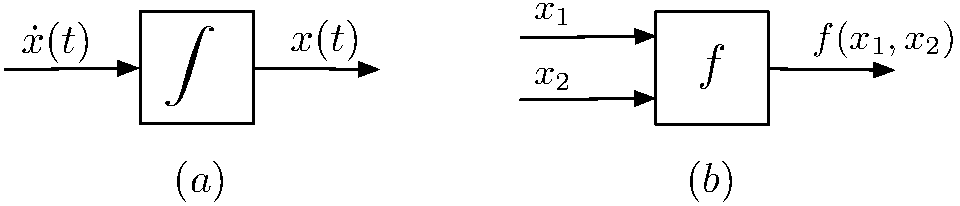
\includegraphics[width=10cm]{blocfonct} 
   \caption{Blocs fonctionnels : (a) intégrateur, (b) fonction}
   \label{Fig:blocfonct}
\end{figure}
\begin{itemize}
\item[$\bullet$] Le bloc fonctionnel Fig. \ref{Fig:blocfonct} 
(a) représente un intégrateur dont la variable d'entrée est 
la dérivée de la variable de sortie.
\item[$\bullet$] Le bloc fonctionnel Fig. \ref{Fig:blocfonct} 
(b) représente une fonction $f: \real^p \rightarrow \real$ dont la variable de 
sortie $z(t)$ est une fonction des variables d'entrée~:
\begin{equation*} \begin{split}
z(t) = f(x_1(t), x_2(t), \dots , x_p(t)).
\end{split} \end{equation*}
\end{itemize}
Dans certains cas, le dessin de ce bloc est particularisé de manière à rendre explicite la fonction qu'il représente. Trois exemples sont indiqués à la figure \ref{Fig:exblocfonct}.  Le schéma fonctionnel d'un système dynamique contient nécessairement $n$ intégrateurs dont les sorties sont les $n$ variables d'état du système. Ces intégrateurs sont interconnectés via des blocs fonctionnels représentant les différentes fonctions apparaissant dans les équations d'état. Les arcs du schéma fonctionnel s'interprêtent comme des lignes de transmission instantanée des variables qui leur sont attachées.
\begin{figure}[htbp] 
   \centering
   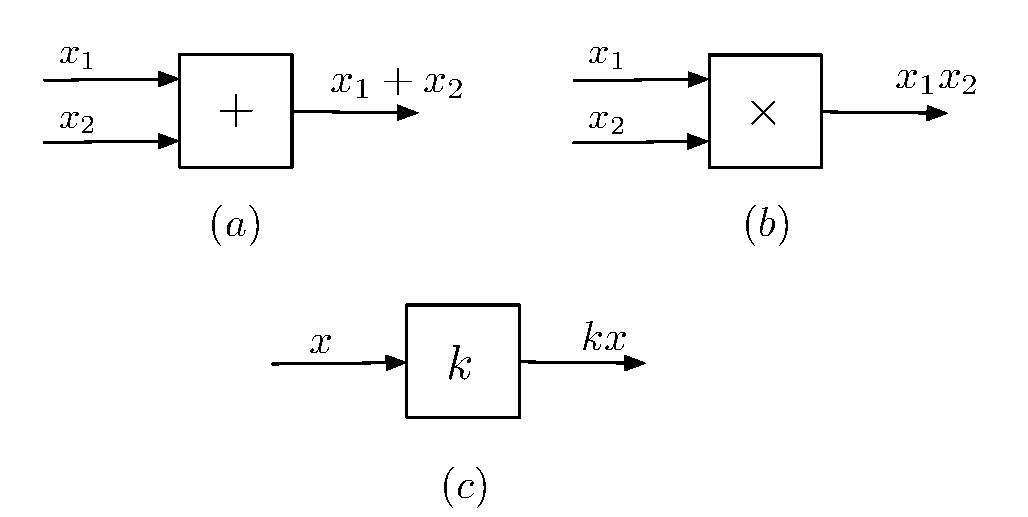
\includegraphics[height=55mm]{exblocfonct} 
   \caption{Exemples de blocs fonctionnels : (a) sommateur, (b) multiplieur, (c) produit par une constante}
   \label{Fig:exblocfonct}
\end{figure}

Outre leur intérêt pour l'analyse des systèmes dynamiques, les 
schémas fonctionnels constituent aussi un outil fondamental de 
programmation dans les langages standard de simulation dynamique 
tels que MATLAB/Simulink ou VisSim.

\begin{exemple}{\bf \em Des algues dans la lagune (suite)}

Au chapitre 5, nous avons établi un modèle simple décrivant la dynamique de croissance d'une population d'algues dans une lagune. En supposant que la cinétique de croissance obéit à une loi bilinéaire $r(x_1,x_2) = x_1x_2$, ce modèle s'écrit~:
\begin{equation*} \begin{split}
\dot x_1 &= -kx_1x_2 + u, \\
\dot x_2 &= x_1x_2 - dx_2.
\end{split} \end{equation*}
Le schéma fonctionnel correspondant est représenté à la figure 
\ref{Fig:schema}. \qed
\begin{figure}[htbp] 
   \centering
   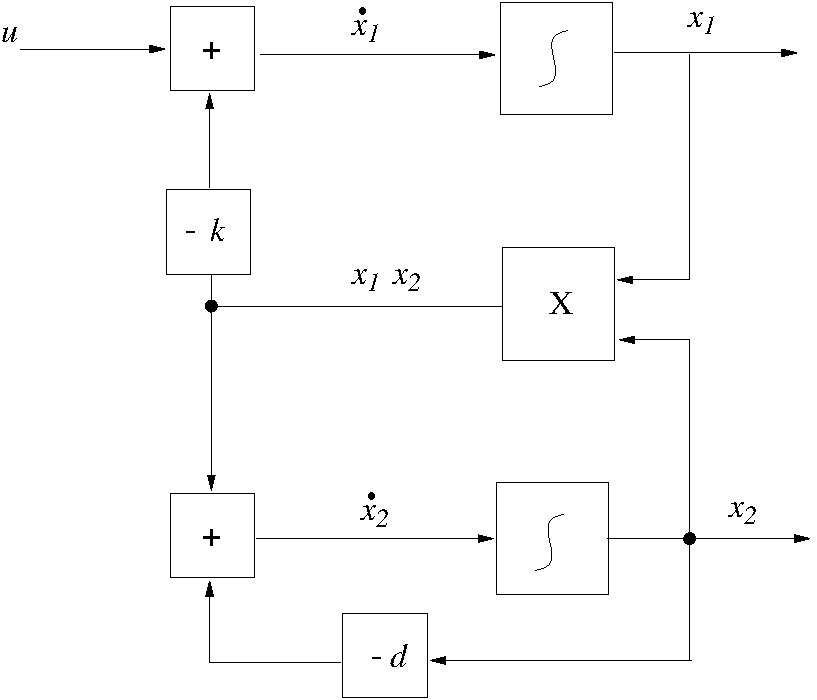
\includegraphics[height=75mm]{schema} 
   \caption{Schéma fonctionnel du modèle de croissance d'algues}
   \label{Fig:schema}
\end{figure}
\end{exemple}

\section{Graphe d'un système dynamique}

Le graphe d'un système dynamique est, d'une certaine manière, le graphe complémentaire du schéma fonctionnel. En effet, ce sont les variables d'état $x_i$ et les variables d'entrée $u_j$ qui sont attachées aux noeuds du graphe tandis que les arcs (orientés) représentent les relations fonctionnelles entre ces variables.

Les règles de construction du graphe d'un système dynamique sont les suivantes~:
\begin{enumerate}
\item Le graphe contient $n+m$ noeuds étiquetés respectivement par les $n$ variables d'état $x_1, x_2, \dots , x_n$ et les $m$ variables d'entrée $u_1,u_2, \dots , u_m$.
\item Il y a un arc orienté de $x_i$ vers $x_j$ (ou de $u_k$ vers $x_j$) si la variable $x_i$ (ou $u_k$) apparait explicitement dans l'équation de la dérivée $\dot x_j$.
\end{enumerate}
\vv

\begin{exemple}{\bf \em Machine électrique à courant continu}

Considérons le modèle général d'une machine DC tel qu'il a été présenté au chapitre 3, section 3.5. C'est un système à quatre variables d'état et 3 variables d'entrée dont le modèle d'état s'écrit~:
\begin{equation*} \begin{split}
\dot x_1 &= x_2, \\
\dot x_2 &= J^{-1}( -h(x_2) + K_mx_3x_4 + u_3), \\
\dot x_3 &= L_f^{-1}(-R_fx_3 + u_1 ), \\
\dot x_4 &= L_a^{-1}(-R_ax_4 - K_ex_2x_3 + u_2).
\end{split} \end{equation*} 
\begin{figure}[htbp] 
   \centering
   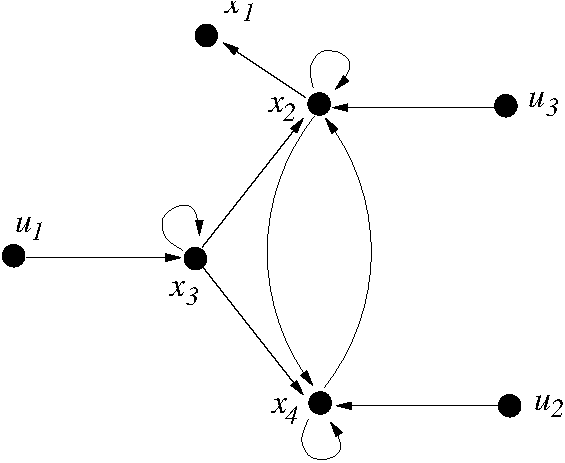
\includegraphics[height=65mm]{grafmot} 
   \caption{Graphe du modèle d'état d'un moteur à courant continu}
   \label{Fig:grafmot}
\end{figure}
Le graphe de ce système est représenté à la figure \ref{Fig:grafmot}. \qed
\end{exemple}
Le graphe d'un système dynamique est un outil permettant de vérifier aisément si le système considéré possède des particularités structurelles intéressantes. Nous en verrons une illustration à la section \ref{triangulaire} lorsque nous étudierons les systèmes triangulaires.

\section{Transformations linéaires d'état}

Pour un système dynamique $\dot x = f(x,u)$, une transformation
linéaire d'état est une application linéaire $T : \real^n
\rightarrow \real^n$ bijective qui transforme l'état du système
$x \in \real^n$ en un nouvel état $z \in \real^n$ selon la règle:
\eqnn
z = Tx
\eeqnn
où $T$ est une matrice $(n \times n)$ régulière.

Dans les nouvelles coordonnées $z$, le modèle d'état du
système est transformé comme suit :
\begin{equation*} \begin{split}
\dot z = T \dot x = Tf(x,u)
\end{split} \end{equation*}
En exprimant que $x= T^{-1}z$ on obtient :
\eqnn
\dot z = g(z,u) \hd \text{avec} \hd g(z,u) \triangleq T f(T^{-1} z,u).
\eeqnn
En particulier, un modèle d'état linéaire $\dot x = Ax + Bu$
est transformé en un autre modèle linéaire :
\eqnn
\dot z = Fz + Gu \hd
\text{avec} \hd F \triangleq TAT^{-1}, \;\;   G \triangleq TB.
\eeqnn

\begin{exemple}{\bf \em Génératrice DC}

Au chapitre 3 (Section 3.6), nous avons établi le modèle d'état d'une
génératrice à courant continu. Lorsque la génératrice tourne à vitesse constante $\omega$, le modèle d'état est linéaire et s'écrit
\eqnn
\bpm
\dot x_1\\ \dot x_2 \epm = 
\bpm
- \dfrac{R_s}{L_s} & 0\\ & \vm \\ 
\dfrac{K_e \omega}{L_r} & - \dfrac{R_r + R_L}{L_r} \epm \bpm x_1\\x_2 \epm +
\bpm \dfrac{1}{L_s} \\ \vm \\ 0 \epm u
\eeqnn
où les variables d'état $x_1$ et $x_2$ représentent respectivement les
courants statorique et rotorique, tandis que l'entrée $u$ est la tension
appliquée au 
circuit statorique.

Nous définissons de nouvelles variables d'état $z_1$ et $z_2$ qui peuvent
être interprétées comme les flux magnétiques $\phi_s$ et $\phi_r$ auxquels
sont soumis
respectivement  les circuits statorique et rotorique :
\begin{equation*} \begin{split}
z_1 &= \phi_s = L_s x_1,\\
z_2 &= \phi_r =  L_r x_2 + K_e x_1.
\end{split} \end{equation*}
On observe qu'il s'agit bien d'une transformation d'état linéaire :
\eqnn
T = \bpm
L_s & 0\\ K_e & L_r \epm.
\eeqnn
La matrice $T$ est inversible (det $T = L_s L_r >0$) et la transformation
inverse s'écrit :
\eqnn
\bpm
x_1 \\x_2 \epm = \bpm \dfrac{1}{L_s} &  0\\ & \vm \\-\dfrac{K_e}{L_sL_r} &
\dfrac{1}{L_r} \epm \bpm z_1\\z_2 \epm.
\eeqnn
Dans les nouvelles coordonnées $(z_1, z_2)$, le modèle d'état s'écrit :
\begin{equation*} \begin{split} 
\bma{c} \dot z_1 \\ \dot z_2 \ema &= \bma{lcc}-\dfrac{R_s}{L_s} & & 0\\ & & \\
\dfrac{K_e\omega}{L_r} + \dfrac{K_e(R_r+R_L)}{L_r L_s}  - 
\dfrac{K_eR_s}{L^2_s} & & -\dfrac{R_r+R_L}{L_r} \ema \bma{c} z_1\\z_2 \ema \\ & \vspace{-4mm} \\ & \hd +
\bma{c} 1 \\ \vspace{-2mm} \\ \dfrac{K_e}{L_s} \ema u \hspace{8cm} \qed
\end{split} \end{equation*}
\end{exemple} 
\vv

\begin{exemple}{\bf \em Modèles linéaires à compartiments}

On s'intéresse ici aux modèles linéaires à compartiments tels que décrits à la section 4.4. Rappelons que la forme générale des équations d'état est la suivante~:
\eqnn
\dot x_i= \sum^n_{j=1} k_{ji} x_j - \sum^n_{\ell=0} k_{i\ell}x_i +b_iu_i, 
\hspace*{10mm} i = 1,n
\eeqnn
ou sous forme matricielle~:
\eqnn
\dot x = Ax + Bu
\eeqnn
avec $A$ une matrice de Metzler diagonalement dominante et $x_i$ la quantité totale contenue dans le compartiment $i$.

On souhaite exprimer le modèle en termes de concentrations.  On introduit les notations :
\begin{equation*} \begin{split}
V_i &: \mbox{ volume du compartiment } i,\\
a_{ij} &\triangleq  k_{ij} V_i,\\
z_i&= \frac{x_i}{V_i} : \mbox{ concentration dans le compartiment } i.
\end{split} \end{equation*}
A l'aide de ces notations, on peut réécrire le modèle comme suit :
\begin{equation*} \begin{split}
\dot x_i &= \sum^n_{j=1} \frac{a_{ji}}{V_j} x_j - \sum^n_{l=0}\frac{a_{il}}{V_i}x_i + b_i u_i,\\
\dot x_i&= \sum^n_{j=1} a_{ji} z_j -\sum_{\ell=0}^n a_{i\ell} z_i + b_i u_i,
\end{split} \end{equation*}
et donc :
\eqnn
\dot z_i = \sum^n_{j=1} \frac{a_{ji}}{V_i} z_j - \sum^n_{\ell=0} \frac{a_{i\ell}}{V_i} z_i + \frac{b_i}{V_i} u_i
\eeqnn
On a opéré ainsi une transformation d'état en passant des quantités  totales $x_i$ aux concentrations $z_i$ comme variables d'état.  Sous forme matricielle la transformation d'état s'écrit :
\eqnn
z = V^{-1}x \mbox{ avec } V \triangleq \mbox{ diag} \{ V_i, i=1, \ldots, n \}
\eeqnn
Dans les coordonnées de concentration, le modèle devient :
\eqnn
\dot z = Fz + Gu
\eeqnn
avec $ F \triangleq V^{-1} AV$ et $ G \triangleq V^{-1} B$.  
On peut vérifier que la matrice $F^T$ est aussi une matrice de Metzler diagonalement dominante.  \qed
\end{exemple}
\vv

\begin{exemple}{\bf \em Diagonalisation et constantes temps}

On considère un modèle linéaire $\dot x = Ax +Bu$ dont la matrice $A$ a
 toutes ses valeurs propres $\lambda_i$ réelles, distinctes et non-nulles.  
 Elle est alors diagonalisable, c'est à dire qu'il existe une matrice
  $T$ telle que
\eqnn
D \triangleq TAT^{-1} = \mbox{ diag}(\lambda_i, i=1, n)
\eeqnn
Si on définit une transformation d'état :
\eqnn
z = Tx
\eeqnn
\noindent le système est transformé en :
\eqnn
\dot z = Dz + TBu
\eeqnn
ou, encore composante par composante :
\eqnn
 \dot z_i = \lambda_i z_i + \beta_i u \;\;\;\; i=1,n
\eeqnn
où $\beta_{i}$ est la i-ème ligne de la matrice $TB$. Les grandeurs
$\tau_i = |\lambda_i|^{-1}, i=1,\ldots , n$, sont les {\em constantes de temps du système}.
\begin{figure}[htbp]    \centering
   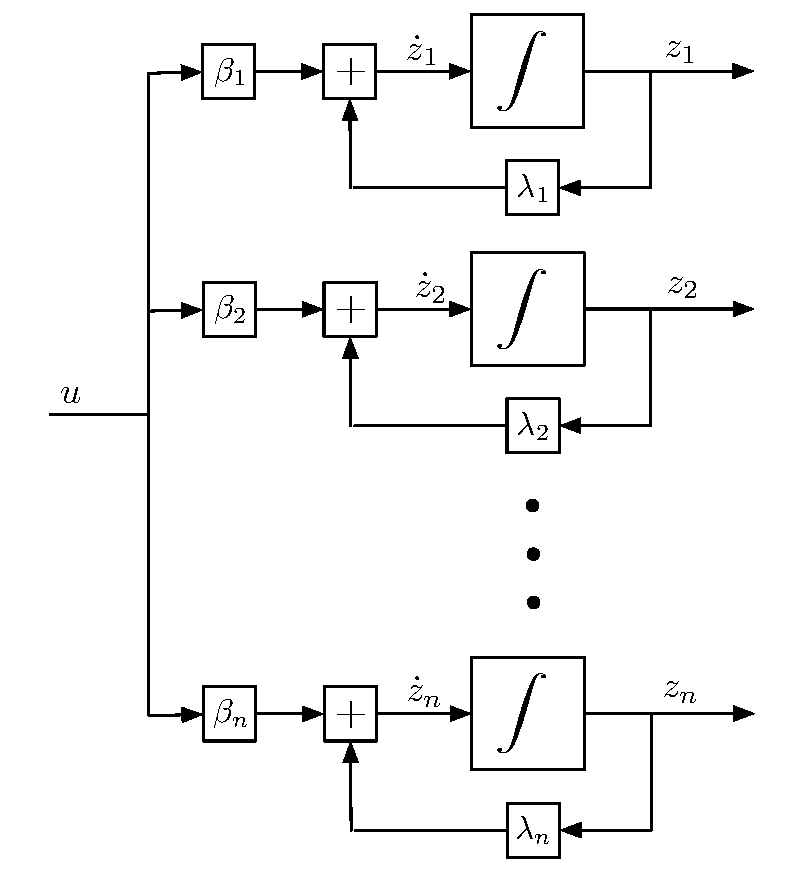
\includegraphics[height=10cm]{schemadiag} 
   \caption{Schéma fonctionnel d'un système diagonalisé à une entrée}
   \label{Fig:schemadiag}
\end{figure}

On a ainsi remplacé le modèle initial dont les variables d'état peuvent être 
fortement couplées, par une collection de systèmes du premier ordre 
complètement séparés les uns des autres comme on peut l'observer sur le schéma fonctionnel de la figure \ref{Fig:schemadiag}.

Par exemple pour un moteur DC commandé par le stator (voir chapitre 3, section 3.6) avec $h(\omega) = B\omega$~:
\eqnn
\dfrac{d}{dt} \bma{c} I_s\\ \omega\ema = \bma{cc}-\dfrac{R_s}{L_s}& 0\\ & \vm \\
\dfrac{K_mI_r}{J} & -\dfrac{B}{J} \ema  \bma{c} I_s\\ \omega\ema +
\bma{c}\dfrac{1}{L_s}u_1\\ \vm \\ \dfrac{1}{J} u_2 \ema,
\eeqnn
on vérifie que les constantes de temps sont 
\begin{equation*} \begin{split}
 \tau_e &= \dfrac{L_s}{R_s}  \text{ constante de temps électrique},\\
\tau_m &= \dfrac{J}{B} \text{ constante de temps mécanique}. \xqedhere{3.5cm}{\qed} 
\end{split} \end{equation*}
\end{exemple}
\vv

\begin{exemple}{\bf \em Systèmes réactionnels sous forme compartimentale}

Au chapitre 5, nous avons vu que le modèle d'état des systèmes réactionnels s'écrit
\eqnn 
\dot x =  Cr(x) + q_{in}(x,u) - q_{out}(x,u).  
\eeqnn
Nous introduisons les notations suivantes pour les vecteurs d'entrée et de sortie :
\begin{equation*} \begin{split}
q_{in}(x,u) &\teq \Big(q_{o1}(x,u), q_{o2}(x,u), \hdots , q_{on}(x,u)\Big)^T, \\
q_{out}(x,u) &\teq \Big(q_{1o}(x,u), q_{2o}(x,u), \hdots , q_{no}(x,u)\Big)^T.
\end{split} \end{equation*}
Supposons que le système est conservatif et que les flux $q_{oi}$ et $q_{io}$ vérifient les conditions C1, C2 et C3 du chapitre 4. Alors le système réactionnel est équivalent à un système à compartiments avec la transformation linéaire d'état :
\eqnn
z = T x, \hd T \teq \textrm{ diag} \{ \omega_2, \omega_2, \hdots , \omega_n \}.
\eeqnn
Pour illustrer cette propriété, considérons à nouveau l'exemple du réacteur chimique parfaitement mélangé de l'exemple 5.6. Dans ce réacteur, les deux réactions 
\begin{equation} \begin{split} \label{exa}
X_1 + X_2 \; &\longrightarrow \; 2X_3, \\ 
2X_3 \; &\longrightarrow \; X_4 
\end{split} \end{equation}
 se déroulent simultanément dans la
phase liquide avec les cinétiques
\begin{equation} \begin{split} 
r_1(x) &= k_1x_1x_2e^{-(Kx_4)}, \\
r_2(x) &= k_2x_3^2. 
\end{split} \end{equation}
Le réacteur est
alimenté par les deux réactifs initiaux $X_1$ et $X_2$ en solution avec des
concentrations d'alimentation
$x_1^{in}$ et $x_2^{in}$.

Le modèle d'état s'écrit
\eqnn
\bpm \dot x_1 \\ \dot x_2 \\ \dot x_3 \\ \dot x_4 \epm =
\bpm -1 & 0 \\ -1 & 0 \\ 2 & -2 \\ 0 & 1 \epm \bpm
k_1x_1x_2e^{-(Kx_4)} \\ k_2x_3^2 \epm 
 + u \bpm x_1^{in} -x_1 \\ x_2^{in} -x_2 \\ -x_3 \\ -x_4
\epm   
\eeqnn
où les variables d'état $x_1, x_2, x_3$ et $x_4$ représentent les
concentrations des différentes espèces dans le milieu réactionnel. 

On vérifie aisément que le système est conservatif avec le vecteur de normalisation $\omega = (1,1,1, 2)$. On définit donc la transformation linéaire d'état
\eqnn
z_1 = x_1, \hd z_2 = x_2, \hd z_3 = x_3, \hd z_4 = 2x_4.
\eeqnn
Dans ces nouvelles coordonnées, on obtient bien un système à compartiments dont le graphe est donné sur la Fig.\ref{reacompart} et dont voici le modèle d'état : 
\eqnn
\bpm \dot z_1 \\ \dot z_2 \\ \dot z_3 \\ \dot z_4 \epm = \bpm -k_1 z_2 \varphi - u & 0 & 0 & 0 \\ 0 & -k_1 z_1 \varphi - u & 0 & 0 \\ k_1 z_2 \varphi & k_1 z_1 \varphi & -2 k_2 z_3 - u & 0 \\ 0 & 0 & 2 k_2 z_3 & -u \epm \bpm z_1 \\ z_2 \\ z_3 \\ z_4 \epm + \bpm u x_1^{in} \\ u x_2^{in} \\ 0 \\ 0 \epm 
\eeqnn
avec
\eqnn
 \varphi \teq \exp(- \dfrac{K}{2} z_4). \xqedhere{5cm}{\qed}
\eeqnn

\end{exemple}
\begin{figure}[tbp] 
   \centering
   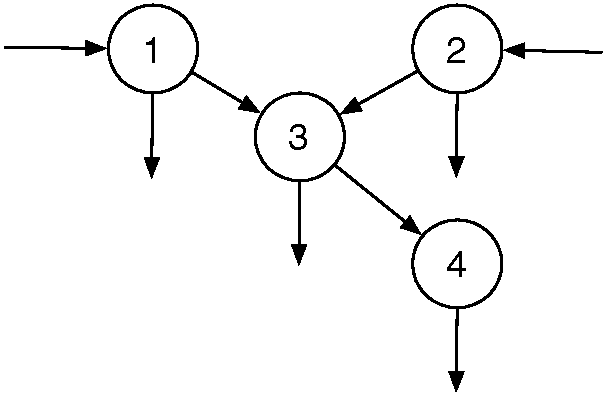
\includegraphics[height=30mm]{reacompart} 
   \caption{Représentation compartimentale d'un système réactionnel}
   \label{reacompart}
\end{figure}


\section{Transformations non linéaires d'état}

Pour un modèle d'état non linéaire $\dot x = f(x,u)$, il est
souvent plus intéressant de considérer des
transformations d'état non linéaires.  Cependant, il n'est
généralement pas possible de définir des transformations {\em
globales} qui soient valables pour tout $x \in \real^n$.  On
s'intéresse dès lors à des transformations {\em locales} qui ne
sont définies que sur des sous-ensembles de $\real^n$.

\begin{definition}{\bf \em Transformation non linéaire d'état}

Soient $U$ et $V$ deux sous-ensembles ouverts de $\real^n$.  Une transformation non linéaire d'état est une application  $T : U
\rightarrow V$ qui transforme l'état du système $x \in U$ en
un nouvel état $z \in V$ :
$$
z = T(x)
$$
et qui possède les propriétés suivantes :
\begin{enumerate}
\item[a)] l'application $T$ est bijective, c'est à
dire qu'il existe une fonction inverse $T^{-1} : V
\rightarrow U$ telle que $x = T^{-1} (z)$,
\item[b)] $T(x)$ et $T^{-1}(z)$ sont des fonctions de
classe $C^{1}$, c'est à dire continues et différentiables.
\end{enumerate}
\noindent La transformation d'état est dite {\em globale} si $U=V=\real^n$. \qed
\end{definition}

Une transformation $T$ possédant ces propriétés 
s'appelle  un difféomorphisme.  La bijectivité de la transformation est nécessaire pour pouvoir inverser le changement de variables d'état et
revenir dans les variables d'état initiales.
La propriété b)  ($T$ et $T^{-1}$ sont de classes $C^1$)
est nécessaire pour pouvoir exprimer le modèle d'état dans les
nouvelles coordonnées comme suit :
$$
\dot z = \frac{\partial T}{\partial x} \dot x = \frac{\partial
T}{\partial x} f(x, u)
$$
où, en utilisant $x = T^{-1}(z)$, on obtient 
$$
\dot z = g(z,u)
$$
avec :
\begin{equation*} \begin{split} 
g(z,u) \triangleq \left[ \frac{\partial T}{\partial x}
f(x,u)\right ]_{x = T^{-1}(z)}.
\end{split} \end{equation*}
De manière similaire, on peut exprimer :
$$
f(x,u) \triangleq \left[\frac{\partial T^{-1}}{\partial z}
g(z,u)\right ]_{z = T(x)}
$$
Les propriétés données dans le lemme suivant peuvent être utiles pour démontrer l'existence d'une transformation d'état non linéaire.
\begin{lemme}{\blanc}
\begin{enumerate}
\item Si la matrice jacobienne $[\partial T/\partial x]$ est régulière au point $x_0$, alors, en application du théorème de la fonction inverse, il existe un voisinage $U$ de $x_0$ tel que l'application $T$ restreinte à $U$ est un difféomorphisme sur $U$.
\item $T$ est un difféomorphisme global si et seulement si~:
\begin{itemize}
\item[a)] $[\partial T/\partial x]$ est régulière pour tout $x$ dans $\real^n$;
\item[b)] $\lim_{\|x\|\rightarrow\infty}\|T(x)\| = \infty$. \qed
\end{itemize}
\end{enumerate}
\end{lemme}

\section{Systèmes mécaniques}

Comme nous l'avons vu au chapitre 2, le vecteur d'état d'un
système mécanique est constitué de deux parties : les
coordonnées de position $q$ et les coordonnées de vitesse
$v=\dot q$
$$ x = \bma{c} q \\ v \ema. $$
Dans de nombreuses applications, il est intéressant de considérer
  différents jeux de coordonnées de position.  La
transformation d'état procède dès lors en deux étapes.  On
transforme tout d'abord les coordonnées de position :
$$ p = \phi (q)$$
où $\phi : U_1 \rightarrow V_1$ est un difféomorphisme et
$\partial \phi /\partial q$ est de plein rang $\forall q \in U_1$.

Le nouveau vecteur d'état est ensuite formé des nouvelles
coordonnées de position $p$ et de leurs dérivées $w = \dot p$ :
$$
z = \bma{c} p\\w \ema.
$$
La transformation d'état est ensuite définie comme suit :
\begin{equation*} \begin{split}
 z = T(x), \hspace*{10mm} \bma{c}p\\w  \ema = \bma{c} \phi(q)\\
\dfrac{\partial \phi}{\partial q} v \ema.
\end{split} \end{equation*}
La transformation d'état inverse est :
$$
x=T^{-1}(z), \hd \bma{c}q\\v \ema = \bma{l} \phi^{-1}(p) \\
\left(\dfrac{\partial \phi}{\partial q}\right )^{-1}_{q = \phi^{-1} p}w
\ema.
$$

\begin{exemple}{\bf \em Coordonnées cartésiennes et polaires}

Dans la méthode décrite au chapitre 2 pour l'établissement
du modèle d'état des systèmes mécaniques articulés, la
position du centre de masse de chaque corps est repérée par ses
coordonnées cartésiennes $q =(x,y)$, comme indiqué sur la figure
\ref{Fig:cocarpol}.
\begin{figure}[htbp] 
   \centering
   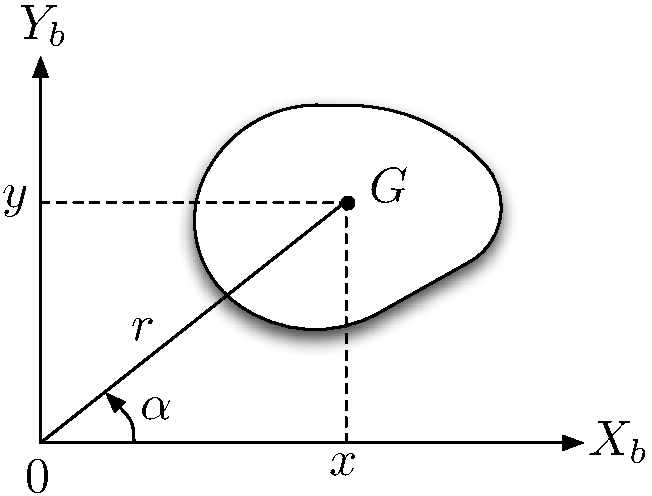
\includegraphics[width=6cm]{cocarpol} 
   \caption{Coordonnées cartésiennes et coordonnés polaires}
   \label{Fig:cocarpol}
\end{figure}
Un autre jeu de coordonnées de position fréquemment utilisées
sont les coordonnées polaires $r$ et $\alpha$ : $r$ est la distance à l'origine du centre de masse et $\alpha$ l'angle entre l'axe $OX_b$ et le
vecteur $\small \overrightarrow{OG}$.

La transformation qui permet de passer des coordonnées
cartésiennes aux coordonnées polaires s'écrit comme suit :
\begin{equation*} \begin{split}
&q = \bma{c} x \\y \ema \;\;\; p = \bma{c} r\\ \alpha \ema,\\
& \vm \\
&p = \phi(q) : \left\{ \begin{array}{ll}
r =&\sqrt{x^2 + y^2},\\ 
\alpha  =&\mbox{arc} \sin \dfrac{y}{\sqrt{x^2 + y^2}} 
\end{array}
\right..
\end{split} \end{equation*} 
La transformation inverse $q = \phi^{-1} (p) $ s'écrit :
\begin{equation*} \begin{split}
x &= r \cos \alpha,\\
y &= r \sin \alpha.
\end{split} \end{equation*}
On observe que le changement de coordonnées $p = \phi(q)$ n'est pas
défini à l'origine, c'est à dire quand $x=0$ et $y=0$.  On
vérifie aussi que 
$$ \det[\frac{\partial \phi^{-1}}{\partial p} ] = r
$$
est nul quand $r=0$ (c'est à dire aussi à l'origine).  Il
s'ensuit que la transformation de coordonnées n'est pas globale
mais valable seulement sur les ensembles suivants:
\begin{equation*} \begin{split}
U_1 &=\real^2 \backslash \{(0,0)\},\\
V_1 &= \real^2 \backslash \{(r, \alpha) : r = 0\}.
\end{split} \end{equation*}
Finalement, la transformation d'état complète entre l'état
$(q,v)$ et l'état $(p,w)$ s'écrit comme suit :
\begin{equation*} \begin{split}
r&= \sqrt{x^2 +y^2},\\
\alpha &= \mbox{arc} \sin \frac{y}{\sqrt{x^2 +y^2}},\\
\dot r &= \frac{x \dot x + y \dot y}{\sqrt{x^2 +y^2}},\\
\dot \alpha &= \frac{x \dot y - \dot x y}{x^2 + y^2},
\end{split} \end{equation*}
et la transformation inverse :
\begin{equation*} \begin{split}
x&= r \cos \alpha,\\
y &= r \sin \alpha,\\
\dot x &= \dot r \cos \alpha - r \dot \alpha \sin \alpha,\\
\dot y &= \dot r \sin \alpha + r \dot \alpha \cos \alpha. \xqedhere{4.6cm}{\qed}
\end{split} \end{equation*}
\end{exemple}

\begin{exemple}{\bf \em Coordonnées articulaires et coordonnées 
de tâche en robotique}

Pour des robots manipulateurs comportant autant d'actionneurs que de degrés de liberté, avec joints rotoïdes,  les coordonnées articulaires du Chapitre 2 constituent des coordonnées \og naturelles \gf pour la description du système : chaque coordonnée repère la position d'un bras par rapport au précédent.  Généralement, avec ces coordonnées, le modèle prend une forme assez simple. Les modèles articulaires conviennent bien pour la conception des systèmes de commande de robots.

Du point de vue de l'utilisateur intéressé par exemple par la planification 
de trajectoires, ce sont cependant les coordonnées de tâche, c'est à dire 
les coordonnées de l'effecteur qui sont intéressantes.  Considérons par 
exemple un robot planaire à deux degrés de liberté se déplaçant dans un 
plan horizontal (voir figure \ref{Fig:robplan}).
\begin{figure}[htbp]
   \centering
   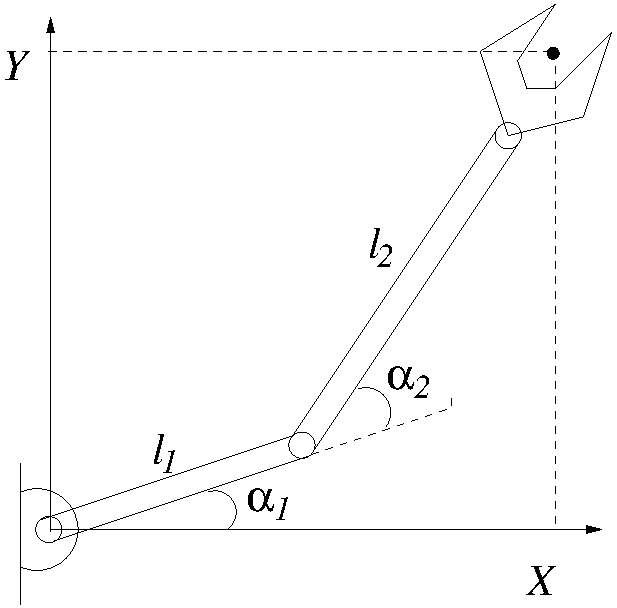
\includegraphics[width=6cm]{robplan} 
   \caption{Coordonnées articulaires et coordonnées de t\^ache d'un robot à 2
degrés de liberté.}
   \label{Fig:robplan}
\end{figure}
Les coordonnées articulaires sont les angles $\alpha_1$ et $\alpha_2$, les 
coordonnées de t\^ache sont les coordonnées cartésiennes $X$ et $Y$.
Nous avons donc : 
$q = (\alpha_1, \alpha_2)$ et $p = \phi(q) = (X,Y)$.  La transformation permettant de
passer des coordonnées articulaires aux coordonnées de t\^ache s'écrit 
\eqn
 X &=& l_1 \cos \alpha_1 + l_2 \cos(\alpha_1 + \alpha_2)\label{artache1},\\
 Y &= &l_1 \sin\alpha_1 + l_2 \sin(\alpha_1 + \alpha_2)\label{artache}.
\eeqn
\noindent On vérifie aisément que cette transformation ne peut pas être injective : à
une position $(X,Y)$ de l'effecteur correspond deux positions distinctes et
symétriques du robot.  Pour définir correctement une transformation de
coordonnées, il faut préciser les domaines $U$ et $V$ de définition de
l'application $\phi$ et de son inverse.

On observe tout d'abord que l'image de l'application $\phi$ est
nécessairement restreinte au disque des positions accessibles par le robot,
c'est à dire (si $l_2 > l_1)$ au disque de rayon $l_1 + l_2$ :
$$ 
V_1 \triangleq \{(X,Y) : (l_2 - l_1)^2 < X^2 + Y^2 < (l_1 + l_2)^2 \}.
$$
D'autre part le domaine de définition de $\phi$ doit être choisi de manière
que l'application soit injective.  Un choix possible est le suivant :
$$
U_1 \triangleq \{(\alpha_1, \alpha_2) : -\pi < \alpha_1 < \pi \;\;\; 0 <
\alpha_2 < \pi\}.
$$
Avec ces définitions, on peut vérifier que l'application 
$$
\phi : U \longrightarrow V
$$
définie par les équations (\ref{artache1})-(\ref{artache}) est un difféomorphisme.

Il reste ensuite à compléter la transformation pour l'étendre aux coordonnées
de vitesses.  Les vecteurs d'état en coordonnées articulaires et en
coordonnées de t\^ache sont définis comme suit : 
$$
x^T = (\alpha_1, \alpha_2, \dot \alpha_1, \dot\alpha_2), \hspace*{10mm} z^T
= (X,Y,\dot X, \dot Y).
$$
La transformation d'état $z = T(x)$ s'écrit finalement comme suit :
\begin{equation*} \begin{split}
X &= l_1 \cos\alpha_1 + l_2 \cos(\alpha_1 + \alpha_2),\\
Y&= l_1 \sin\alpha_1 + l_2 \sin(\alpha_1 + \alpha_2,\\
\dot X &=-l_1 \dot \alpha_1\sin\alpha_1 -l_2 \dot \alpha_1\sin(\alpha_1+\alpha_2) - l_2 \dot \alpha_2\sin(\alpha_1 + \alpha_2),\\
\dot Y &= l_1 \dot \alpha_1\cos\alpha_1 + l_2 \dot \alpha_1\cos(\alpha_1+\alpha_2) + l_2 \dot \alpha_2\cos(\alpha_1 + \alpha_2). \xqedhere{1.8cm}{\qed}
\end{split} \end{equation*}
\end{exemple}

\section{Machines électriques}

Au chapitre 3, nous avons obtenu un modèle  général des machine électriques tournantes de la forme suivante :
\begin{equation*} \begin{split}
L(\theta) \dot I &= -\omega K(\theta) I - RI +V, \\
\dot\theta &= \omega, \label{machel}\\
J \dot \omega &= \frac{1}{2}I^TK(\theta)I - h(\omega) + T_a, 
\end{split} \end{equation*}
avec
$$
K(\theta)\triangleq\frac{\partial L(\theta)}{\partial \theta}.
$$
Ces équations conduisent naturellement à établir des modèles d'état dont le
vecteur d'état
$$
x^T = (I^T, \theta, \omega)
$$
est composé des courants $I$, de la position angulaire $\theta$ et de la 
vitesse angulaire $\omega$.  D'autres choix de variables d'état peuvent être
utilisés pour faciliter l'étude mathématique des machines électriques.
Une transformation courante consiste à remplacer les courants par les flux :
$$
\phi = L(\theta)I,
$$
c'est à dire à tranformer le vecteur d'état $x^T = (I^T, \theta, \omega)$ en
le vecteur d'état $z^T = (\phi^T, \theta, \omega)$.  Cette transformation est bien un difféomorphisme car la matrice d'inductances
$L(\theta)$ est inversible pour tout $\theta$.

Dans les nouvelles variables d'état $z$, les équations (\ref{machel}) se
réécrivent : 
\begin{equation*} \begin{split}
\dot\phi &= -RL^{-1}(\theta)\phi+ V,\\
\dot \theta &= \omega,\\
J\dot\omega &= \dfrac{1}{2} \phi^T G(\theta) \phi - h(\omega) + T_a,\\
\mbox{ avec } G(\theta) &\triangleq  L^{-1}(\theta)K(\theta)L^{-1}(\theta).
\end{split} \end{equation*}
\vv

\section{Systèmes triangulaires} \label{triangulaire}
 
 Un système à {\it une seule} entrée (système mono-entrée)
 \eqn
 \dot x = f(x,u) \hh \hh x \in \real^n \hh \hh u \in \real \label{mono}
 \eeqn
est dit {\it triangulaire} s'il vérifie la définition suivante.

\begin{definition}{\bf \emph Système triangulaire}

Un système dynamique mono-entrée est triangulaire si il existe une variable d'état $x_i$ telle que le plus court chemin allant de $u$ à $x_i$ dans le graphe du système est de longueur $n$. \qed
\end{definition}

Pour un système triangulaire, il est dès lors toujours possible de renuméroter les variables d'état de telle sorte que le modèle d'état s'écrive comme suit~:
\begin{equation} \begin{split} \label{systriang}
\dot x_1 &= g_1(x_1,x_2),  \\
\dot x_2 &= g_2(x_1,x_2, x_3),  \\
&\vdots  \\
\dot x_i &= g_i(x_1,x_2, \dots ,x_{i+1}),  \\
&\vdots  \\
\dot x_{n-1} &= g_{n-1}(x_1,x_2, \dots ,x_n),  \\
\dot x_n &= g_n(x_1,x_2, \dots ,x_n,u).  
\end{split} \end{equation}
On observe que le nombre de variables d'état apparaissant à droite augmente progressivement de $2$ à $n$ (d'où le nom de forme triangulaire). En outre, l'entrée $u$ n'apparait que dans la dernière équation.
\vv

\begin{exemple}{\bf \em Robot manipulateur à un degré de liberté avec une articulation élastique \label{exrobot}}

Le modèle d'état d'un robot manipulateur à un degré de liberté avec une articulation rotoïde élastique et des couples de frottement négligeables s'écrit~:
\begin{equation} \begin{split} \label{robotelast}
\dot x_1 &= x_2,  \\
J_1\dot x_2 &= -mgd\sin x_1 - k(x_1 - x_3),  \\
\dot x_3 &= x_4,  \\
J_2\dot x_4 &= k(x_1 - x_3) + u.
\end{split} \end{equation}
où

$x_1$ est la coordonnée angulaire de position du bras,

$x_2$ est la vitesse angulaire du bras,

$x_3$ est la coordonnée de position angulaire du moteur,

$x_4$ est la vitesse angulaire du moteur,

$J_1$ et $J_2$ sont les moments d'inertie du bras et du moteur,

$d$ est la distance entre l'articulation et le centre de masse,

$k$ est la constante de rappel élastique,

$u$ est le couple de commande développé par le moteur.\\

\noindent Le graphe du système est représenté à la figure 
\ref{Fig:grafrobot} et on peut vérifier que les équations d'état possèdent bien la structure triangulaire voulue. \qed
\begin{figure}[htbp]
   \centering
   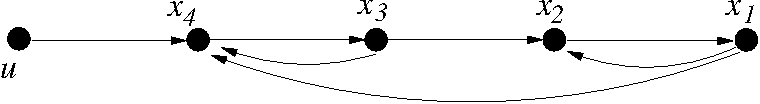
\includegraphics[width=9cm]{grafrobot} 
   \caption{Graphe du modèle d'un robot à un bras avec articulation élastique.}
   \label{Fig:grafrobot}
\end{figure}
\end{exemple}

\section{Forme canonique de Brunovski} \label{sectionbrunovski}

\begin{definition}{\blanc}

Un système dynamique mono-entrée (\ref{mono}) est sous forme canonique de Brunovski si il existe
 une tranformation d'état $ T : U \rightarrow V$ et un intervalle ouvert $W \subset \real$ 
  tels que, dans les nouvelles variables d'état $z=T(x)$, le système prends la forme triangulaire particulière suivante~:
 \begin{equation*} \begin{split}
 \dot z_1 &= z_2,\\
 \dot z_2 &= z_3,\\
 \vdots &\\
 \dot z_n &= \alpha (z_1, z_2, \ldots, z_n, u),
\end{split} \end{equation*}
où la fonction $\alpha$ est continue et inversible par rapport à $u$ sur $W$ pour tout $z \in V$.
\qed
\end{definition}

 On observe que le système est ainsi constitué d'une cha\^{i}ne d'intégrateurs
 de la forme
 \begin{equation*} \begin{split}
 \dot z_i = z_{i+1}\;\;\; i = 1. \ldots, n-1
 \end{split} \end{equation*}
 et que toute les nonlinéarités du système sont concentrées dans la seule
 fonction nonlinéaire scalaire $\alpha (z_1, z_2, \ldots, z_n, u)$.  La forme
 canonique de Brunovski peut aussi être schématisée comme indiqué sur le schéma fonctionnel de la
 figure \ref{Fig:bruno}. La forme de Brunovski est intéressante parce qu'elle permet d'effectuer facilement des planifications de trajectoire comme nous le verrons au chapitre 10.
  \begin{figure}[htbp] 
    \centering
    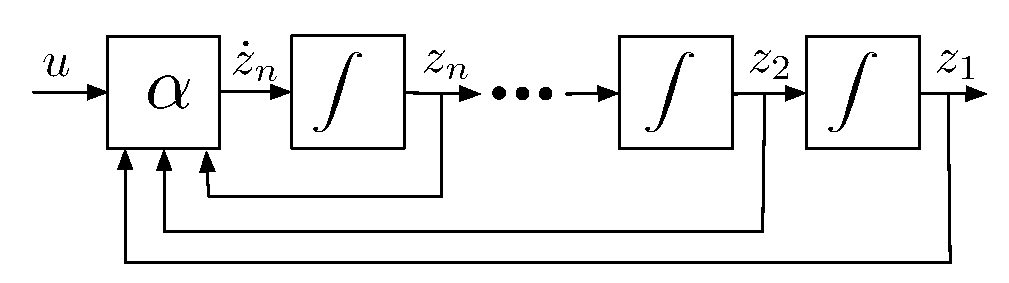
\includegraphics[width=9cm]{bruno} 
    \caption{Schéma fonctionnel de la forme canonique de Brunovski}
    \label{Fig:bruno}
 \end{figure}
 
\begin{exemple}{\bf \em Un réacteur chimique \label{exreachim} }
 
On considère un réacteur continu parfaitement mélangé et à volume
constant dans lequel se déroule une réaction chimique irréversible mettant
 en oeuvre deux espèces $X_1$ et $X_2$ :
 $$
 X_1 \longrightarrow X_2.
 $$
 Le réacteur est alimenté uniquement avec l'espèce $X_1$, à concentration
 $c$ constante.  La variable d'entrée est le débit volumétrique spécifique
 d'alimentation du réacteur.  La cinétique obéit à la loi d'action des
 masses.  Selon les principes de modélisation que nous avons établi au
 chapitre 5, on obtient le modèle d'état bilinéaire suivant :
 \begin{equation*} \begin{split}
 \dot x_1 &= -kx_1 + u (c-x_1),\\
 \dot x_2 &= kx_1 - ux_2.
 \end{split} \end{equation*}
 On définit la transformation d'état $z = T(x)$ suivante :
 \begin{equation*} \begin{split}
 z_1 &= \frac{x_2}{c-x_1},\\
 z_2 &= \frac{kx_1(c-x_1-x_2)}{(c-x_1)^2}.
 \end{split} \end{equation*}
 Le domaine $U$ et l'image $V$ de l'application $T : U \longrightarrow V$
 sont définis comme suit :
 \begin{equation*} \begin{split}
 U &= \{(x_1, x_2) : x_1 > 0, x_2 > 0, x_1+x_2 < c \},\\
 V &= \{(z_1,z_2) : 0<z_1 <1, z_2>0 \}.
 \end{split} \end{equation*}
On peut
 alors montrer que la transformation d'état $z = T(x)$ ainsi définie est bien
 un difféomorphisme dont l'inverse est :
 \begin{equation*} \begin{split} 
 x_1 &= \frac{cz_2}{k(1-z_1)+z_2},\\
 x_2 &= \frac{ckz_1(1-z_1)}{k(1-z_1)+z_2}.
 \end{split} \end{equation*}
 Dans les nouvelles coordonnées, le modèle d'état est sous forme canonique de
 Brunovski :
 \begin{equation*} \begin{split} 
 \dot z_1 &= z_2,\\
 \dot z_2 &= -\left( z_2 + \dfrac{(k+1)z^2_2}{k(1-z_1)} \right) + (k(1-z_1) + z_2)u.
 \end{split} \end{equation*} 
La fonction $\alpha$ est inversible par rapport à $u$ sur $W$. \qed
\end{exemple}

Cet exemple montre qu'il n'est pas évident de déterminer a priori si un système dynamique donné peut être mis sous forme de Brunovski ni de déduire la transformation d'état adéquate. Cependant, si le système concerné est déjà donné sous forme triangulaire, une condition suffisante pour le mettre sous forme de Brunovski s'exprime comme suit.
\begin{lemme}{\blanc} \label{lemmeici}

Un système dynamique triangulaire décrit par le modèle d'état (\ref{systriang}) peut être mis sous forme canonique de Brunovski au voisinage de $(x_0,u_0)$ si les inégalité suivantes~:
\begin{equation*} \begin{split}
\frac{\partial g_i}{\partial x_{i+1}} &\neq 0 \hh \hh i=1, \ldots, n-1, \\
\frac{\partial g_n}{\partial u} &\neq 0,
\end{split} \end{equation*}
sont satisfaites en $(x_0,u_0)$.
\qed
\end{lemme}
\vv

\begin{exemple}{\bf \em Robot manipulateur à un degré de liberté avec articulation élastique (suite)}

On considère à nouveau le modèle (\ref{robotelast}) de l'exemple \ref{exrobot}. On vérifie aisément que les conditions du Lemme \ref{lemmeici} sont satisfaites pour tout $x \in \real^4$ et conduisent naturellement à la transformation d'état~:
\begin{equation*} \begin{split} 
z_1 &= x_1 \\
z_2 &= x_2 \\
z_3 &= -J_1^{-1}[mgd\sin x_1 + k(x_1 -x_3)] \\
z_4 &= -J_2^{-1}[mgdx_2 \cos x_1 + k(x_2 - x_4)].
\end{split} \end{equation*}
La transformation inverse s'écrit~:
\begin{equation*} \begin{split} 
x_1 &= z_1 \\
x_2 &= z_2 \\
x_3 &= (mgdk^{-1} \sin z_1 + z_1 + J_1k^{-1}z_3) \\
x_4 &= (mgdk^{-1} z_2 \cos z_1 + z_2 + J_2k^{-1}z_4) 
\end{split} \end{equation*}
On observe qu'il s'agit d'un difféomorphisme global de $\real^4$ dans $\real^4$. Avec les nouvelles variables d'état le modèle s'écrit sous forme de Brunovski~:
\begin{equation*} \begin{split} 
\dot z_1 &= z_2 \\
\dot z_2 &= z_3 \\
\dot z_3 &= z_4 \\
\dot z_4 &= J_2^{-1}[mgd(z_2^2 \sin z_1 - z_3 \cos z_1) -k z_3] \\ & \hh \hh + kJ_2^{-2}[mgd\sin z_1 + J_1z_3 - u]
\end{split} \end{equation*}
On observe aussi que la fonction $\alpha$ est inconditionnellement inversible sur $\real$ par rapport à $u$. La forme de Brunovski est donc ici globalement valide. \qed
\end{exemple}
Pour des systèmes qui ne sont pas donnés sous forme triangulaire mais qui sont affines en l'entrée, le lemme suivant exprime des conditions utiles pour trouver la transformation d'état.
\begin{lemme}{\blanc}
Un système affine en l'entrée
$$
\dot x = f(x) + g(x)u \hh \hh x \in \real^n \hh \hh u \in \real
$$
peut être mis sous forme canonique de Brunovski dans un domaine $U \subset \real^n$ si il existe une transformation d'état $z = T(x)$ vérifiant les conditions suivantes~:
\begin{equation*} \begin{split} 
& T_{i+1}(x) = \frac{\partial T_i}{\partial x}f(x) \hh \hh i=1,2, \ldots, n-1, \\
& \frac{\partial T_i}{\partial x}g(x) = 0 \hh \hh i=1,2, \ldots, n-1, \\
& \frac{\partial T_n}{\partial x}g(x) \neq 0,
\end{split} \end{equation*}
pout tout $x \in U$. \qed
\end{lemme}
\vv

\begin{exemple}{\bf \em Un réacteur chimique (suite)}

Nous montrons comment utiliser le lemme précédent pour retrouver la transformation d'état qui a été postulée sans justification dans l'exemple \ref{exreachim}. Le modèle d'état s'écrit~:
\begin{equation*} \begin{split}
\bma{c} \dot x_1 \\ \dot x_2 \ema = \bma{c} -x_1 \\ x_1 \ema + \bma{c} c-x_1 \\ -x_2 \ema u \triangleq f(x) + g(x)u
\end{split} \end{equation*}
On considère tout d'abord l'équation aux dérivées partielles~:
\begin{equation*} \begin{split}
\frac{\partial T_1}{\partial x}g(x)=0 \hh \Rightarrow \hh \frac{\partial T_1}{\partial x_1}(c-x_1) = \frac{\partial T_1}{\partial x_2}x_2
\end{split} \end{equation*}
dont une solution est~:
\begin{equation*} \begin{split}
T_1(x) = \frac{x_2}{c-x_1}
\end{split} \end{equation*}
On calcule ensuite~:
\begin{equation*} \begin{split}
T_2(x) = \frac{\partial T_1}{\partial x}f(x) \hh \Rightarrow \hh T_2(x) = \frac{kx_1(c-x_1-x_2)}{(c-x_1)^2}
\end{split} \end{equation*}
On détermine le domaine $U$ et l'image $V$ de l'application $T:U \rightarrow V$ ainsi définie. On vérifie enfin que la condition $(\partial T_2/\partial x)g(x) \neq 0$ est satisfaite sur $U$~:
\begin{equation*} \begin{split}
\frac{\partial T_2}{\partial x}g(x) = \frac{c(c-x_1-x_2)}{(c-x_1)^2} \neq 0 \xqedhere{3.9cm}{\qed}
\end{split} \end{equation*}
\end{exemple}

\section{Exercices}

\begin{exercice}{\bf \em Un four de verrerie}

Au Chapitre 1, Exemple 1.1 et Exercice 1.1, nous avons proposé trois jeux différents de variables d'état pour un modèle de four de verrerie. Déterminer les trois transformations d'état correspondantes et indiquer leurs domaines de définition. \qed
\end{exercice}
\vv


\begin{exercice}{\bf \em Un relais electromagnétique}

Soit le relais électromagnétique dont le modèle d'état à été
établi au Chapitre 3, Exemple 3.2.
\begin{enumerate}
\item On choisit les nouvelles variables d'état suivantes : $y_1 = z$,
$y_2 = \dot z$, $y_3 = \phi(I,z)$. Montrer qu'il s'agit d'une
transformation d'état valide. Etablir le modèle d'état dans ces
nouvelles variables.
\item Montrer que le système peut être mis sous forme canonique de
Brunovski. Déterminer la transformation d'état et donner une
interprétation physique des nouvelles variables d'état. \qed
\end{enumerate}
\end{exercice}
\vv

\begin{exercice}{\bf \em Une cage d'ascenseur}

\begin{tabular}{p{6.5cm}p{2mm}c}
\vspace{-3.2cm} 
Sur la figure ci-contre, on a représenté une cage d'ascenseur suspendue à un cable élastique de masse négligeable.
\vspace{2mm}

\noindent {\bf Notations :}

$y$ = longueur du câble

$\omega$ = vitesse angulaire de la poulie

$R$ = rayon de la poulie

$m$ = masse de la cage

\vspace{2mm}
\noindent La tension dans le câble est modélisée par la loi de Hooke :
\begin{equation*}
T = \frac{k(y - z)}{z}
\end{equation*}
où $z$ est une variable d'état auxiliaire dont la dérivée est la vitesse périphérique de la poulie : $\dot z = R \omega$.
& &
\parbox[c]{6cm}
{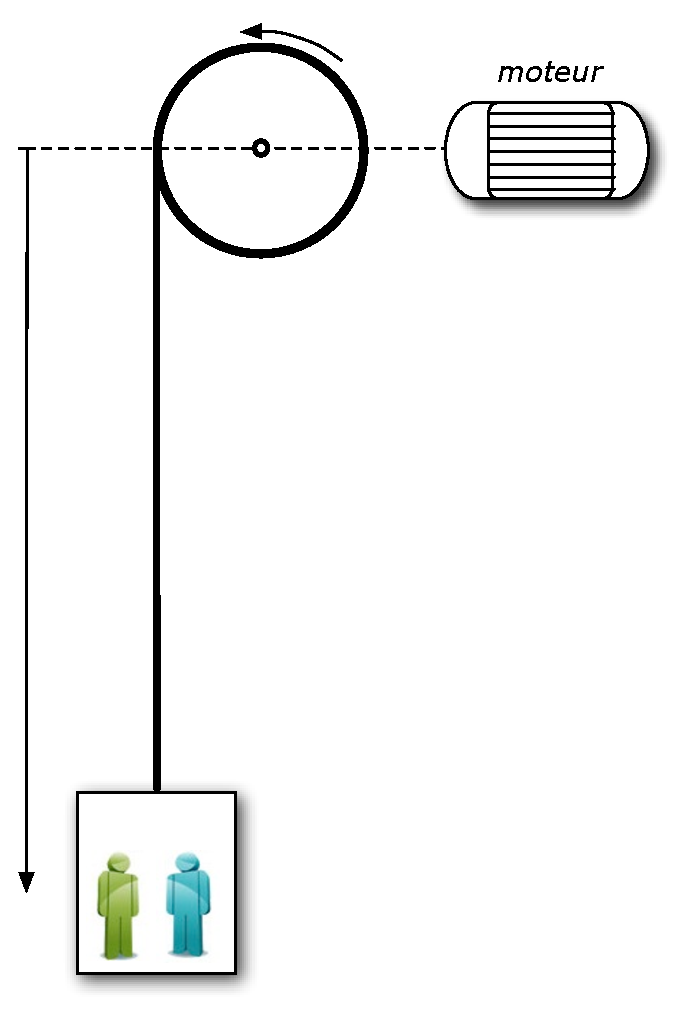
\includegraphics[width=4.5cm]{ascenseur.pdf}}
\end{tabular}

\begin{enumerate}
\item Etablir un modèle d'état avec 4 variables d'état : $y, \dot y, z, \omega$. Le frottement est négligé. La variable d'entrée est le couple de rotation $u$ appliqué à la poulie.
\item Montrer que le système peut être mis sous forme de Brunovski. Expliciter la transformation d'état. \qed
\end{enumerate}
\end{exercice}
\vv

\begin{exercice}{\bf \em Des coccinelles et des pucerons}

Montrer qu'il existe une transformation d'état telle que le système (\ref{coc}) du chapitre 1 modélisant l'interaction entre les populations de coccinelles et de pucerons peut être mis sous la forme d'un système à compartiments. Dessiner le graphe associé. Déterminer les flux $q_{ij}$, la matrice $L$ et la matrice $A(x,u)$. \qed
\end{exercice}
\vv

\begin{exercice}{{\bf \em Un réacteur biochimique}}

Soit un réacteur continu parfaitement mélangé et à volume
constant dans lequel se déroule une réaction chimique autocatalytique
irréversible mettant en oeuvre deux espèces $A$ et $B$~:
\e
A + B \longrightarrow 2B
\ee
Le réacteur est alimenté uniquement avec l'espèce $A$, à
concentration constante. La variable d'entrée est le débit
volumétrique d'alimentation du réacteur. Les cinétiques obéissent
à la loi d'action des masses. 
\begin{enumerate}
\item Etablir les équations d'état du système.
\item Montrer que le système est conservatif.
\item Déterminer une transformation d'état qui mette le
système sous forme canonique de Brunowski.
\item Déterminer la transformation d'état qui met le système sous la forme d'un système à compartiments.
\item Mêmes questions si la réaction est réversible. \qed
\end{enumerate}
\end{exercice}
\vv

\begin{exercice}{\bf Un four électrique}

Un four électrique est chauffé par une thermistance comme indiqué sur la figure ci-dessous.
\begin{figure}[h]
\begin{center}
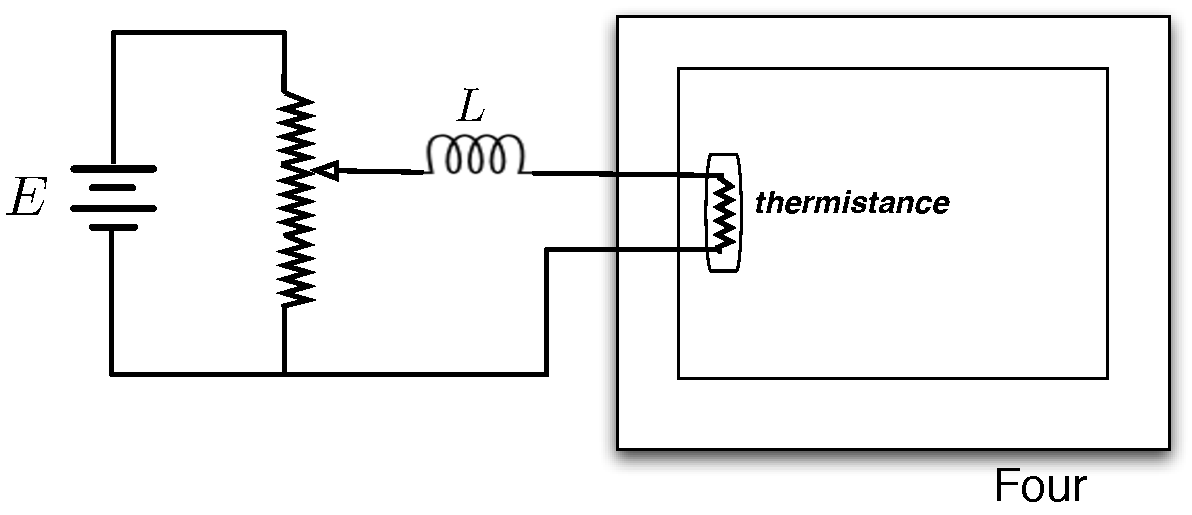
\includegraphics[width=8cm]{four}
\label{four}
\end{center}
\vspace{-5mm}
\end{figure}
\begin{enumerate}
\item Etablir un modèle d'état du système sous les hypothèses de modélisation suivantes :
\begin{itemize}
\item[a)] La thermistance est une résistance dont la valeur varie avec la temperature suivant la relation de Reinhart-Hart :
\begin{equation*}
\dfrac{1}{T} = a + b \ln R + c (\ln R)^3
\end{equation*}
où $a, b, c$ sont des constantes caratéristiques positives fournies par le constructeur.
\item [b)] Comme représenté sur la figure, la thermistance est alimentée par une batterie de tension constante $E$ via une inductance (linéaire) constante et une résistance (linéaire) règlable qui est l'entrée du système.
\item[c)] Le four est chauffé par la thermistance. La perte de chaleur à travers les parois du four est proportionnelle à la différence  entre la température à l'intérieur du four et la température extérieure qui est supposée constante. 
\end{itemize}
\item Montrer que le système peut être mis sous forme de Brunovski. Expliciter la transformation d'état. \qed
\end{enumerate}
\end{exercice}
\vv

\begin{exercice}{\bf \em Un système à deux compartiments}

Soit le système {\em linéaire} à deux compartiments dont le graphe
est indiqué à la figure \ref{Fig:deuxcomp}. Déterminer la transformation d'état qui diagonalise le
système. Expliciter les constantes de temps. \qed
\begin{figure}[h] 
   \centering
   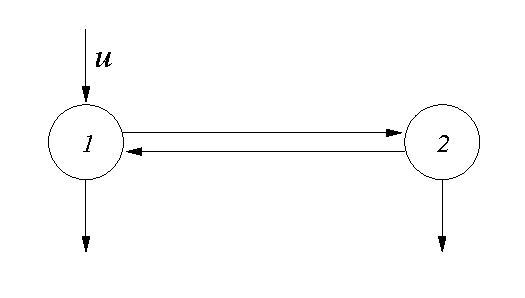
\includegraphics[width=6cm]{deuxcomp} 
   \caption{Graphe d'un système à deux compartiments}
   \label{Fig:deuxcomp}
\end{figure}
\end{exercice}

\end{document}